\pagebreak
\section{Inertia Test}
\nopagebreak
%\subsection{} %\label{put a label here and uncomment}
\textbf{Name: Group 510}\\
\textbf{Date: 02/11 - 2015}

\subsubsection{Purpose}
The purpose of the test is to measure the inertia of the loaded vehicle $J_{tot}$.

\subsubsection{Setup}
\begin{figure}[H]
	\centering
	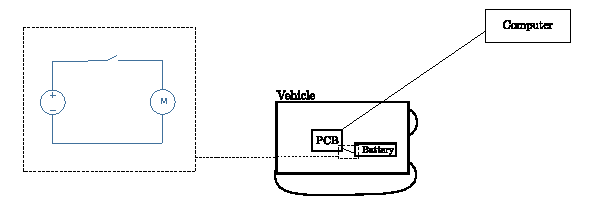
\includegraphics[scale=1.6]{figures/inertiaTestSetupDiagram.pdf}
	\caption{Setup diagram}
	\label{inertiaTestSetupDiagram}
\end{figure}

\subsubsection{List of Equipment}

\begin{table}[H]
\begin{tabular}{|p{10cm}|p{4cm}|}
\hline%------------------------------------------------------------------------------------
  \textbf{Instrument}                     &  \textbf{Type}       \\
\hline%------------------------------------------------------------------------------------
  Computer                                &  Asus N73JN    \\
\hline %-----------------------------------------------------------------------------------
\end{tabular}
\end{table}


\subsubsection{Procedure}

\begin{enumerate}
  \item Connect the vehicle to the computer via the arduino card, and disconnect the battery.
  \item Upload the test code to the Arduino board the Arduino IDE (see \cite{ArduinoIDE}).
  \item Open a serial terminal via PuTTY (see \cite{PuTTY}). All the measured data is retrieved from that terminal.
  \item Plug in the battery so the vehicle runs.
  \item After a few seconds, the code cuts the power of the motor by sending a PWM with 0\% duty cycle to let the speed decrease progressively. An alternative is to unplug the motor's power channel from the PCB.
  \item Wait until the vehicle stops to end measuring the speed of it.
  \item Plot the speed of the vehicle.
\end{enumerate}

\subsubsection{Results} \label{inertiaTestResults}

The \figref{inertiaTestPowerCutOrDisable} shows the vehicle's velocity variations throughout time, both when the motor is unplugged manually or when its power is cut via software :

\begin{figure}[H]
  \centering
  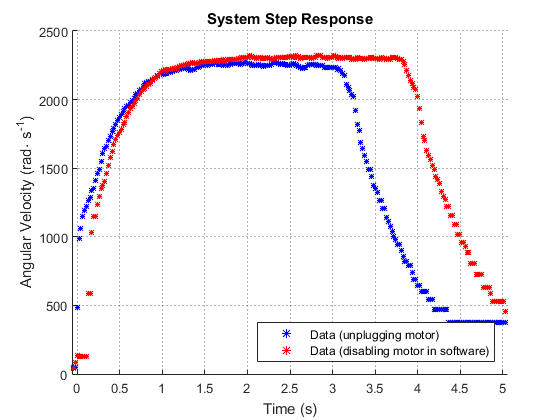
\includegraphics[scale=0.7]{figures/inertiaTestPowerCutOrDisable.png}
  \caption{Plot of the inertia measured speed of the vehicle over time when the motor is unplugged and when it is disabled via software.}
  \label{inertiaTestPowerCutOrDisable}
\end{figure}
%
By comparing both methods to cut off the motor's power, the back electromotive force generated by the motor when using the software method seems negligeable since both curves have very similar decreasing shapes. Moreover, the manual unplugging of the powering wires brings some uncertainty due to a potential distrubing force applied to the vehicle.
Therefore, the software method is used to extract the inertia.

\begin{figure}[H]
  \centering
  %\includegraphics[scale=0,5]{figures/InertiaTestPlot.pdf}
  \caption{Plot of the inertia measured speed of the vehicle over time.}
  \label{intertiaTestPlot}
\end{figure}